%%
%% Beuth Hochschule für Technik --  
%%
%% Kapitel 7 - 
%%
%%	

\newpage

[Burde]
\section{Simulation des Regelkreises mit dem entworfenen Regler} \label{Kapitel7}

Der entworfene PI-Regler soll nun in einer Simulation des Regelkreises getestet werden. Dabei sollen folgende Punkte betrachtet werden:

\begin{itemize}
\item Aussteuerbereich der Stellgröße

\item Führungsverhalten

\item Störverhalten
\end{itemize}

Dazu wird nun ein Simulink Modell erstellt, in welchem die komplette Regelstrecke als Modell nachgebaut wird. 

\begin{figure}[h]
	\begin{center}
		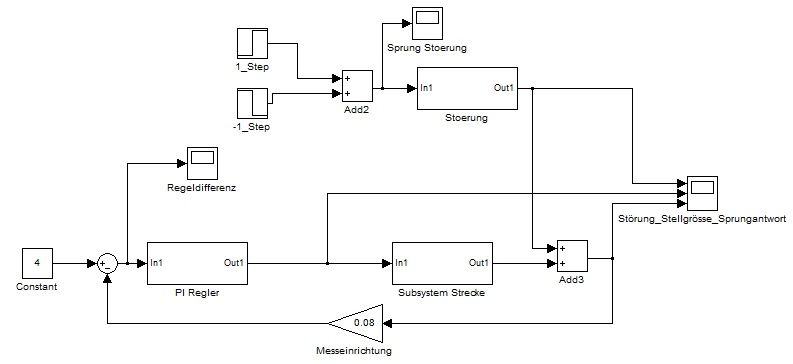
\includegraphics[scale=0.7]{simulink_modell.jpg}
		\caption{Simulink Modell des Regelkreises}
       \label{simulink}
	\end{center} 
\end{figure}

Die Strecke, der Regler sowie die Störung sind jeweils in Subsysteme untergebracht. Nachdem die Strecke mit einem $4V$ Sprung in den Arbeitsbereich gebracht wird, folgt nach der 4,5 Sekunde eine Störung, die nach der 9 Sekunde wieder ausgeschaltet wird. In Abbildung \ref{scope_simu} ist nun die Störung, die Stellgröße sowie die Sprungantwort des Regelkreises dargestellt.

\newpage

\begin{figure}[h]
	\begin{center}
		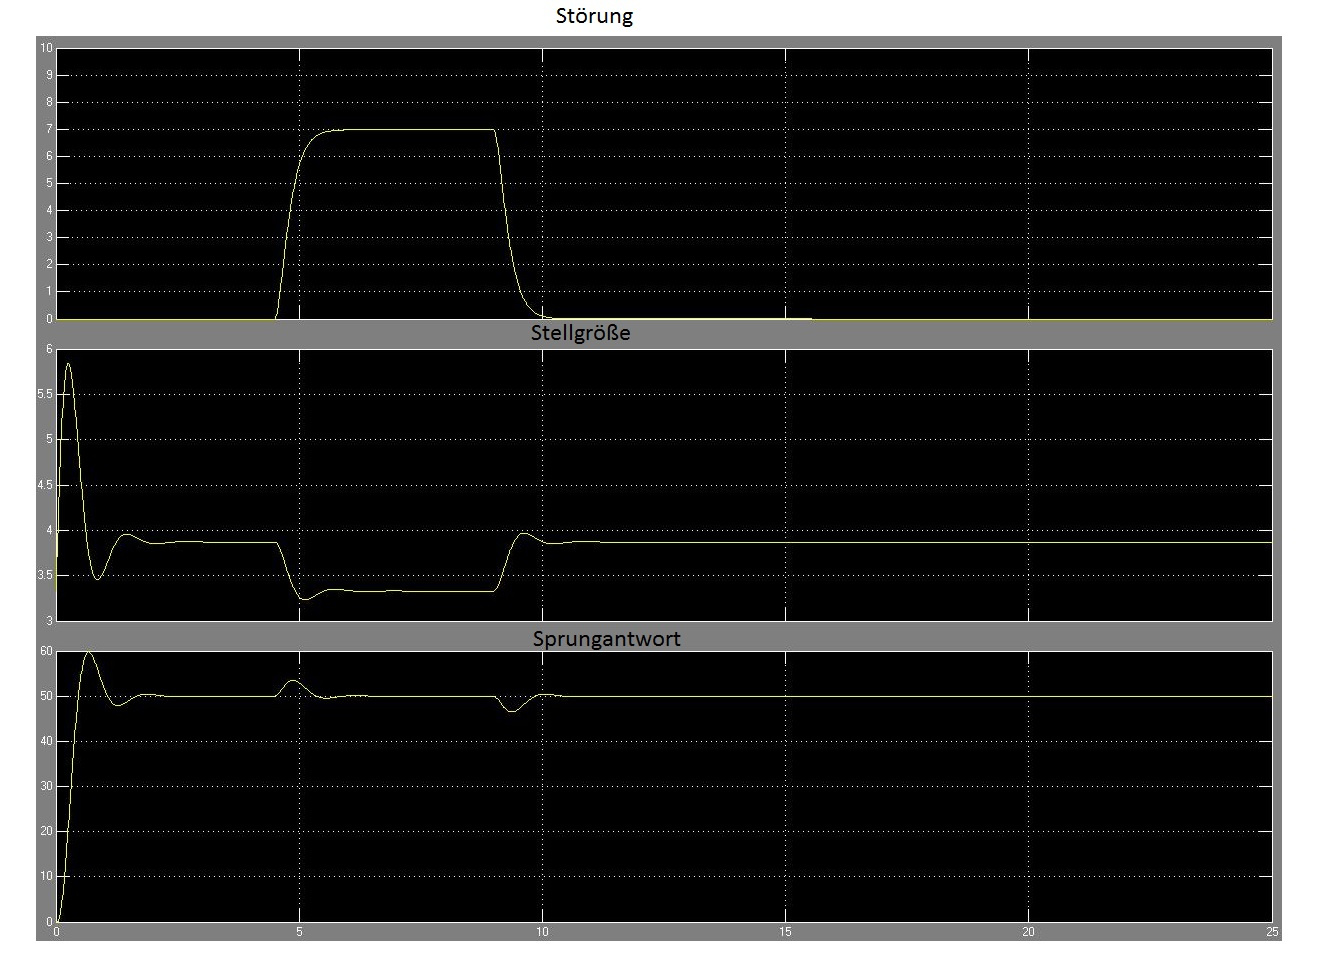
\includegraphics[scale=0.4]{scopes_simu.jpg}
		\caption{Störung, Stellgröße und Sprungantwort des Regelkreises mit Regler}
       \label{scope_simu}
	\end{center} 
\end{figure}

Anhand der Abbildung lassen sich einige Schlussfolgerungen zum Regelkreis aufstellen. Die Stellgröße übersteuert nicht und bleibt im Bereich zwischen $0V$ und $10V$. Anhand der Sprungantwort lässt sich feststellen, dass die maximal erlaubte Überschwingweite von 20 Prozent nicht überschritten wird. Diese liegt hier beim Einschaltvorgang bei 10 Bar. Erlaubt wären maximal 12 Bar. Auch eine bleibende Regelabweichung lässt sich in der Sprungantwort nicht ermitteln. Somit kann im nächsten Kapitel die Implementierung des Reglers in die reale Strecke vorgenommen werden.

